\subsubsection{Verwendete Pakete}
„Softwarepakete sind Sätze von Programmdateien, Bibliotheken und anderen Ressourcen, die Softwareentwicklern helfen sollen, Anwendungen zu erstellen. Sie bieten eine Grundlage von vorgefertigtem Code und Komponenten, die Entwickler verwenden können, um schnell Anwendungen zu erstellen, ohne den Code von Grund auf neu schreiben zu müssen.“ \citev{pakete} \\ \\
Beim Erstellen der App mithilfe von Expo sind folgende Pakete bereits vorinstalliert:\\
\begin{itemize}
  \item expo
  \item expo-status-bar
  \item react
  \item react-native
  \item expo-updates
\end{itemize}
Jedoch werden für die Entwicklung der App viele weitere Pakete benötigt. Expo bietet zwar viele integrierte Funktionen und Bibliotheken, aber es gibt immer noch einige Szenarien, in denen zusätzliche Bibliotheken erforderlich sind, um bestimmte Funktionen zu implementieren.\\
So ist zum Beispiel für die Verwendung von Firebase und der Navigation, die Einbindung von externen Paketen notwendig.\\
In anderen Fällen werden Pakete verwendet, da es die Entwicklung vereinfacht. Ein Beispiel dafür ist das Paket Moment, welches zum Umwandeln von Zeitstempel verwendet wird.\\
Folgende Pakete werden zusätzlich für die Entwicklung der App verwendet:\\


\paragraph{react-native-switch-selector}\mbox{}\\
Version: 2.3.0\\ Quelle: https://www.npmjs.com/package/react-native-switch-selector\\ \\
Dieses Paket wird für den Switch-Selector auf dem Screen Tower verwendet. \\
\begin{figure}[H]
  \centering
  
\includegraphics[width=0.15\textwidth]{images/app-screenshots/switchselector.png}
  
\includegraphics[width=0.15\textwidth]{images/app-screenshots/switchselector2.png}
  \caption{Switch-Selector in der App}
  \label{fig:switchselector}
\end{figure}

\paragraph{Moment}\mbox{}\\
Version: 2.29.4\\ Quelle: https://momentjs.com/\\ \\
In Firebase werden die Zeitpunkte der Einlagerung als \Gls{Unix-Timestamp} gespeichert. Moment erleichtert die Umwandlung vom \Gls{Unix-Timestamp} zu einem Datum mit Uhrzeit. Es wird bei der Anzeige der Einlagerungs- und Auslagerungszeiten verwendet. \\

\paragraph{Geolib}\mbox{}\\
Version: 3.3.3\\ Quelle: https://github.com/manuelbieh/geolib/blob/master/CHANGELOG.md\\ \\
Bei diesem Paket wird die Methode GetPreciseDistance verwendet, um die Distanz zwischen der anwendenden Person und dem Fahrradturm zu berechnen. \\
\begin{listing}[H]
  \begin{minted}{js}
    let distance = getPreciseDistance(
    {
    latitude: userlocation.coords.latitude,
    longitude: userlocation.coords.longitude,},
    { 
    latitude: tower.location.latitude, 
    longitude: tower.location.longitude }
    );
\end{minted}
  \caption{Verwendung der Methode getPreciseDistance}
  \label{lst:getprecisedistance}
\end{listing}
Der Code zeigt die Anwendung der Methode GetPreciseDistance. Dabei werden die Koordinaten der anwendenden Person und des Turmes übergeben. Die Methode liefert die Distanz zwischen den zwei Punkten in Meter.

\paragraph{expo-location}\mbox{}\\
Version: 15.0.1\\
Quelle: https://docs.expo.dev/versions/latest/sdk/location/ \\ \\
Expo-location ermöglicht es auf die GPS-Koordinaten des verwendeten Gerätes zuzugreifen. Dies wird verwendet, um sicherzustellen, dass sich die anwendende Person in der Nähe des Fahrradturmes befindet. \\


\paragraph{Firebase}\mbox{}\\
Version: 9.15.0\\
Quelle: https://docs.expo.dev/guides/using-firebase/\\ \\
Von dieser Bibliothek werden die Methoden auth und firestore verwendet.
\subparagraph{Auth}steht für Authentifizierung. Es wird bei der Entwicklung der App für folgende Zwecke verwendet:
\begin{itemize}
  \item Erstellen von Account
  \item Anmelden mit Account
  \item Abmelden
  \item Zugriff auf ID der anwendenden Person
\end{itemize}

\subparagraph{Firestore}wird für das Schreiben und Lesen von Daten aus der Datenbank verwendet. Dies wird für folgende Zwecke benötigt:
\begin{itemize}
  \item Ausgabe der gelagerten Gegenstände
  \item Anzeige der Fahrradtürme
  \item Einlagerungs- und Auslagerungsprozess
\end{itemize}

\paragraph{react-native-maps}\mbox{}\\
Version: 1.3.2\\
Quelle: https://github.com/react-native-maps/react-native-maps\\ \\
Mit React-native-maps kann man eine Karte auf dem jeweiligen Gerät erzeugen und Marker setzen. Es werden die Komponenten <Mapview> für die Karte und <Marker> für den \Gls{Location-Pin} verwendet.  \\
\begin{figure}[H]
  \centering
  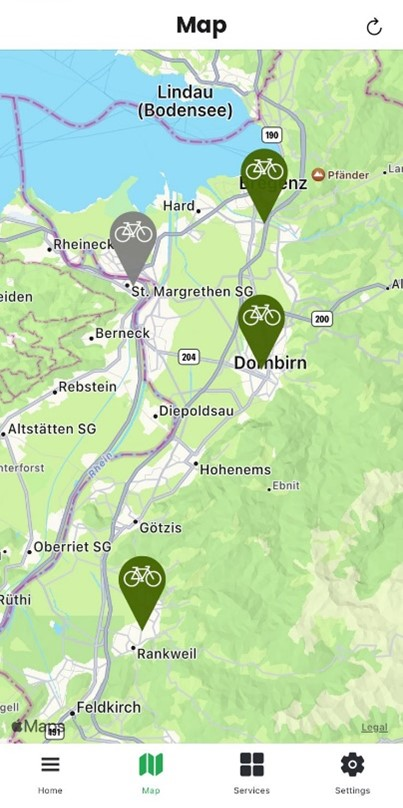
\includegraphics[width=0.2\textwidth]{images/app-screenshots/tabmap.jpg}
  \caption{Karte im Tab „Map“}
  \label{fig:tabmap}
\end{figure}
Wie auf der Abbildung \ref*{fig:tabmap} ersichtlich, wird bei der App die Bibliothek react-native-maps für die Karte mit den Möglichkeiten zum Lagern eines Fahrrades verwendet. \\
\begin{figure}[H]
  \centering
  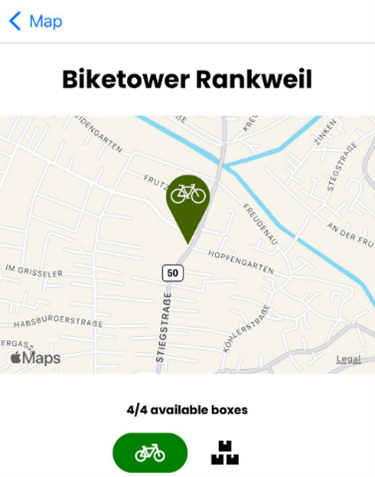
\includegraphics[width=0.2\textwidth]{images/app-screenshots/smallmap.png}
  \caption{Karte im Tab „TowerInfo“}
  \label{fig:smallmap}
\end{figure}
Die Abbildung \ref{fig:smallmap} zeigt die zweite Karte, die im Screen „TowerInfo“ verwendet wird, wo der Standort des Turmes angezeigt wird.\\


\paragraph{react-navigation/native}\mbox{}\\
Version: 6.1.4\\
Quelle: https://reactnavigation.org\\ \\
React-navigation/navtive ist ein Paket, das Teil des React Navigation-\Gls{Framework}s ist. Das Paket wird verwendet, um die Navigation zu initialisieren. Zusätzlich beinhaltet es die Methode getFocusedRouteNameFromRoute. Damit bekommt man den Namen des Screens, auf dem sich die anwendende Person befindet.\\
\begin{listing}[H]
  \begin{minted}{js}
    const routeName = getFocusedRouteNameFromRoute(route);
    if (routeName === "assignment"){
        navigation.setOptions({tabBarStyle: {display: 'none'}});
        
    }else {
        navigation.setOptions({tabBarStyle: {display: 'flex'}});
    }
\end{minted}
  \caption{Verwendung der Methode getFocusedRouteNameFromRoute}
  \label{lst:getfocusedroutename}
\end{listing}
Der Code zeigt die Verwendung der Methode getFocusedRouteNameFromRoute. Falls sich die anwendende Person auf dem Screen Assignment befindet, wird die untere TabBar nicht angezeigt.\\


\paragraph{react-navigation/native-stack}\mbox{}\\
Version: 6.9.7\\
Quelle: https://github.com/software-mansion/react-native-screens\#readme\\ \\
Dieses Paket ist eine Erweiterung von react-navigation/native und wird für den StackNavigator verwendet. Es ermöglicht eine einfache und unkomplizierte Lösung zum Navigieren.
\begin{listing}[H]
  \begin{minted}{js}
    <Stack.Navigator
      screenOptions={({ route }) => ({ 
        headerTitleStyle: {
          fontFamily: "Poppins",
          fontWeight: "400",
        fontSize: 21
      }})}>
      <Stack.Screen name="map" options={{ title: 'Map' }} component={Map} />
      <Stack.Screen name="tower" options={{ title: '' }} component={TowerInfo} />
      <Stack.Screen name="boxinfo" options={{ title: '' }} component={BoxInfo} />
      <Stack.Screen name="assignment" options={{headerShown: false, title: '' }} 
      component={Assignment} />
    </Stack.Navigator>
\end{minted}
  \caption{Verwendung vom StackNavigator}
  \label{lst:stacknavigator}
\end{listing}
Der abgebildete Code zeigt den StackNavigator. Er beinhaltet Optionen für den Header. Jeder einzelne Screen hat einen Namen, einen Titel und eine Komponente.\\


\paragraph{react-navigation/bottom-tabs}\mbox{}\\
Version: 6.5.2\\
Quelle: https://github.com/react-navigation/react-navigation\#readme\\ \\
Mit diesem Paket lässt sich einfach ein TabNavigator erstellen. Das Paket bietet eine Vielzahl von Konfigurationsoptionen für Tabs, damit zum Beispiel der Tab auf dem man sich befindet, hervorgehoben wird.\\

\paragraph{expo-splash-screen}\mbox{}\\
Version: 0.17.5\\
Quelle: https://docs.expo.dev/versions/latest/sdk/splash-screen/\\ \\
expo-splash-screen ist ein Paket, das Teil der Expo \Gls{SDK} ist und zur Verwendung eines Splash-Screens in React Native-Anwendungen verwendet wird. Ein Splash-Screen ist ein Startbildschirm, der beim Starten der Anwendung angezeigt wird, um dem Benutzer visuelles Feedback zu geben, dass die App geladen wird.\\
Das Paket wird beim Screen „Map“ verwendet, wo beim Laden der Türme aus firestore eine leere Karte angezeigt wird.\\


